\section{Sensoren}

\subsection{Übersicht der Hardware}
Die Wetterstation Arbon verfügt über vier Sensoren bzw. Sensor-Einheiten: Webcam, Kombi-Wetter-Transmitter, Wassertemperatur-Sensor und Pegelsensor. Auf der Plattform im See draussen befindet sich lediglich ein Schaltschrank mit Datenwandlern und keine Auswerteeinheit. Sämtliche Daten werden per TCP/IP an den Server geschickt. Abbildung \ref{img:schaltschrank} zeigt den schematischen Aufbau der Komponenten im Schaltschrank und die angeschlossenen Sensoren. Die Stromversorgung ist der Übersicht halber nicht dargestellt.

\begin{figure}[h]
	\centering
	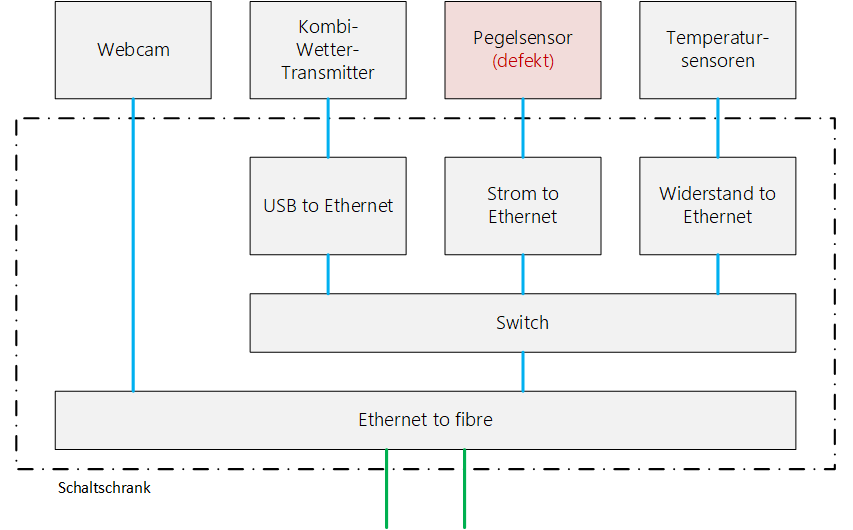
\includegraphics[width=0.9\linewidth]{img/schaltschrank.png}
	\caption{Hardware-Aufbau der Wetterstation Arbon}
	\label{img:schaltschrank}
\end{figure}

%% ###################################################################################################
%%   Unterkapitel                                                                                                                                                                              #
%% ###################################################################################################
\subsection{Pegelsensor und Wellenhöhenmessung}
\Diskussionspunkt{Pegelmessung, Pegelberechnung, Wellenhöhenberechnung}
\Diskussionspunkt{Gegenüberstellung Messprinzipien, Vor- und Nachteile}
\Diskussionspunkt{Unterschied Wellenhöhe und Seegang}

Für die Messung des Bodensee-Pegels wurden verschiedene Messprinzipien verglichen, mit dem Hintergedanken die Pegelmesswerte ebenfalls zur Messung der Wellenhöhe verwenden zu können.

\begin{table}[htb!]
\setlength\extrarowheight{3pt} % for a more "open" look
\begin{tabularx}{\textwidth}{|>{\RaggedRight\hspace{0pt}}p{1.5cm}||X|X|}
\hline
 & \bfseries\large Vorteile & \bfseries\large Nachteile\\

\hline
\textbf{Hydrostatisch}
&
\begin{itemize}[nosep,leftmargin=*]
\item einfache Auswertung
\item mechanische Dämpfung
\item sehr kleiner Energieverbrauch
\end{itemize}
&
\begin{itemize}[nosep,leftmargin=*]
\item anfällig auf Verschmutzung
\item keine Wellenmessung möglich
\end{itemize}\\

\hline
\textbf{Ultraschall}
&
\begin{itemize}[nosep,leftmargin=*]
\item berührungslos
\item geringer Energiebedarf
\end{itemize}
&
\begin{itemize}[nosep,leftmargin=*]
\item anfällig auf Wind
\end{itemize}\\

\hline
\textbf{Radar}
&
\begin{itemize}[nosep,leftmargin=*]
\item windunabhängig
\item berührungslos
\end{itemize}
&
\begin{itemize}[nosep,leftmargin=*]
\item zu geringe Auflösung für Wellenhöhe
\item hoher Energiebedarf
\end{itemize}\\

\hline
\textbf{TOF}
&
\begin{itemize}[nosep,leftmargin=*]
\item Wellenhöhe messbar
\item berührungslos
\end{itemize}
&
\begin{itemize}[nosep,leftmargin=*]
\item komplexe Auswertung
\end{itemize}\\

\hline
\textbf{Boje}
&
\begin{itemize}[nosep,leftmargin=*]
\item Wellenhöhe messbar
\end{itemize}
&
\begin{itemize}[nosep,leftmargin=*]
\item wartungsintensiv
\item Batteriebetrieb
\end{itemize}\\


\hline
\end{tabularx}
\end{table}

\subsubsection{Pegelberechnung}
Der Pegelsensor liefert 4...20mA bei einer Messhöhe von 6 Meter. Der Pegelsensor ist ??? Meter über dem Pegelnullstand (Definition!!!) angebracht.
Für die Berechnung des Bodensee-Pegels aus dem Messwert ergibt sich analog der Geradengleichung $ y = m * x + q  $ wie in der Formel \ref{eq:Pegelformel} dargestellt.

\begin{equation}
\label{eq:Pegelformel}
Pegel [m] = 6m/16mA * Messwert [mA] + ???m
\end{equation}

\Diskussionspunkt{Wie ist der Bodenseepegel definiert? Quelle?}


%% ###################################################################################################
%%   Unterkapitel                                                                                                                                                                              #
%% ###################################################################################################
\subsection{Strahlungssensor}
\Diskussionspunkt{Ziel: Sonnenstunden messen? Wen interessieren die Sonnenstunden?}
\Diskussionspunkt{Wann reicht Globalstrahlung, wann wird Direktstrahlung benötigt?}
\Diskussionspunkt{Was kann auf PV-Berechnungstools eingegeben werden?}

Die Sonnenscheindauer dient der näherungsweisen Abschätzung der Einstrahlung an einem bestimmten Ort und gibt gleichzeitig Hinweise auf Zeit und Stärke der Bewölkung. Die tatsächliche Sonnenscheindauer ist als die Zeitspanne definiert, während der die direkte Sonnenstrahlung senkrecht zur Sonnenrichtung mindestens 120 W/m2 beträgt.
Die effektiv mögliche Sonnenscheindauer wird durch Landschaftshorizonte verkürzt, sodass die Sonnenscheindauer im Dezember in gewissen Tälern im Gebirge sogar Null betragen kann.
Die relative Sonnenscheindauer beschreibt den Anteil der tatsächlichen an der effektiv möglichen Sonnenscheindauer in Prozent. Durch sie kann man Sonnenscheinverhältnisse verschiedener Gebiete vergleichen.

\subsubsection{Auswahl der Hardware}

\Diskussionspunkt{Bild Funktionsweise eines Pyranometers}
\Diskussionspunkt{Foto Hukseflux}

Das Pyranometer basiert auf dem Messprinzip eines Thermoelements. Die eintreffende Strahlung trifft auf einen Absorber, welcher erwärmt wird. Die Wärme „fliesst“ dann über das Gehäuse an die Umgebung ab. Die Strahlungsleistung ist proportional zum Wärmestrom bzw. zur Temperaturdifferenz vom Absorber zum Gehäuse. Die Temperaturdifferenz wird mit Thermoelementen gemessen. Um die Signalspannung zu erhöhen werden mehrere Thermoelemente in Reihe geschalten, welches Thermosäule genannt wird. Durch das thermische Messprinzip ist ein Pyranometer träge. Die Response time liegt bei wenigen Sekunden. Das schwarz-poröse Absorbermaterial muss eine hohe Langzeitstabilität insbesondre gegenüber kurzwelliger Strahlung aufweisen. Das spektrale Verhalten wird durch den Glasdom definiert. Bei Glas liegt dieser im Bereich von 350 bis 2800 nm. Durch Erhöhung der Güte des Doms (Quarzglas) kann der spektrale Bereich erweitert werden von 300 bis 3600 nm. Für Pyranometer existiert ein Standard nach WMO: ISO 9060, mit folgenden Güteklassen:


\begin{itemize}
\item Secondary Standard
\item first class
\item second class
\end{itemize}

\Diskussionspunkt{ISO 9060:1990 Solar energy -- Specification and classification of instruments for measuring hemispherical solar and direct solar radiation}

Die Serie SR05 ist die preiswerteste Serie von Pyranometern, die die Anforderungen der zweiten Klasse nach ISO 9060 erfüllt. SR05 misst die von einer ebenen Fläche empfangene Sonnenstrahlung in W/m2 aus einem Blickwinkel von 180 Grad. Es ist ideal für allgemeine Sonnenstrahlungsmessungen in (agro-)meteorologischen Netzen und PV-Monitoring. Das Pyranometer ist einfach zu montieren und zu installieren, insbesondere mit dem Kugelausgleichsmechanismus des SR05. Zur einfachen Integration stehen verschiedene digitale und analoge Ausgänge zur Verfügung.


\subsubsection{Berechnung der Sonnenstunden}
Zur Messung der Sonnenstunden gibt es gemäss  \flqq Guide to Meteorological Instruments and Methods of Observation\frqq ~\cite{WMO2014Gtmi}  fünf Messprinzipien, wobei die pyranometrische Methode, die einfachste und kostengünstigste Methode darstellt. Die physikalische Größe der Sonnenscheindauer (SD) ist Zeit. Die verwendeten Einheiten sind Sekunden oder Stunden.
Der Messzeitraum (Tag, Dekade, Monat, Jahr usw.) ist ein wichtiger Zusatz zur Einheit.


Pyranometrische Methode: Pyranometrische Messung der globalen Sonneneinstrahlung $G$ zur Abschätzung der Sonnenscheindauer. Art des Instruments: Ein Pyranometer in Kombination mit einem elektronischen oder computergesteuerten Gerät, das in der Lage ist 1 Minute globale Sonneneinstrahlung $G$ zu liefern.


Gemäss ANNEX 8.B. der Richtlinie ~\cite{WMO2014Gtmi} kann die Sonnenscheindauer aus den minütlichen Messwerten der Globalstrahlung berechnet werden. Dazu muss zuerst der Schwellwert, wie in \ref{eq:Sonnenstunden} dargestellt, berechnet werden. Der Zähler für die Sonnenstunden wird um eine Minute erhöht, wenn der Messwert grösser ist als der Schwellwert und der Sonnenwinkel mindestens 3 Grad beträgt.

\begin{equation}
\label{eq:Sonnenstunden}
G_{thr} = A + B * cos(\frac{360*d}{24*365}) * 1080 * sin(h)^{1.25}
\end{equation}

wobei:
\begin{conditions}
$G_{thr}$  &  Schwellwert der Globalstrahlung \\
$d$        &  Laufende Stunde seit Anfang Jahr \\
$h$        &  Elevationswinkel der Sonne in Grad \\
$A$        &  Empirisch bestimmter Koeffizient (0.65) \\
$B$        &  Empirisch bestimmter Koeffizient (0.15) \\
\end{conditions}

Wenn der Winkel $h$ grösser oder gleich 3 Grad ist, und der gemittelte Minutenwert der Solarstrahlung höher ist als der Schwellwert, wird der Zähler für die Sonnenstunde um eine Minute erhöht.

Guten Tag Frau Bilgery,
scheint grössere Abweichungen zu geben. Habe es mit zwei anderen Datensätzen versucht mit dem ähnlichen Ergebnis.

Im beiliegenden File habe ich die Strahlung bei einer Sonnenhöhe <3° auf Null gesetzt, d.h. Morgen und Abendstunden werden nicht berücksichtigt. Fehler mit Division von sin(h) gibt es dann auch nicht.
Für Buchs ist dies zulässig da die umliegenden Berge über einem Höhenwinkel von 3° liegen. Dies wird aber in der Literatur auch für südliche Regionen ohne Berge durchgeführt. D.h. dies ist eine Massnahme. Weitere Massnahme ist die Reduktion der Faktoren A und B bis die Werte übereinstimmen.

Faktor B-Reduktion kann beurteilt werden, wenn ein Sommertag und Wintertag betrachtet wird, da dieser die Saisonalität bestimmt.


%% ###################################################################################################
%%   Unterkapitel                                                                                                                                                                              #
%% ###################################################################################################
\subsection{Wassertemperatur-Sensoren}
\Diskussionspunkt{Berechnung, Verlauf der Wassertemperatur in Abhängigkeit der Tiefe}
\Diskussionspunkt{Welcher Sensor muss auf Grund des Pegels ausgewählt werden -> Skizze}
\Diskussionspunkt{Offset des defekten Sensors -> Grafik}

\subsubsection{Auswahl des richtigen Temperatursensors}
Um die richtige Temperaturen bestimmen zu können ist der Pegel notwendig, hierfür wird im Cronjob zuerst den Pegel ausgelesen und anschliesend mittels der if Funktion, dies musste mit einem if gemacht werden, da Python keine cases kennt, den richtigen Sensor ausgewählt.

\begin{figure}[h]
	\centering
	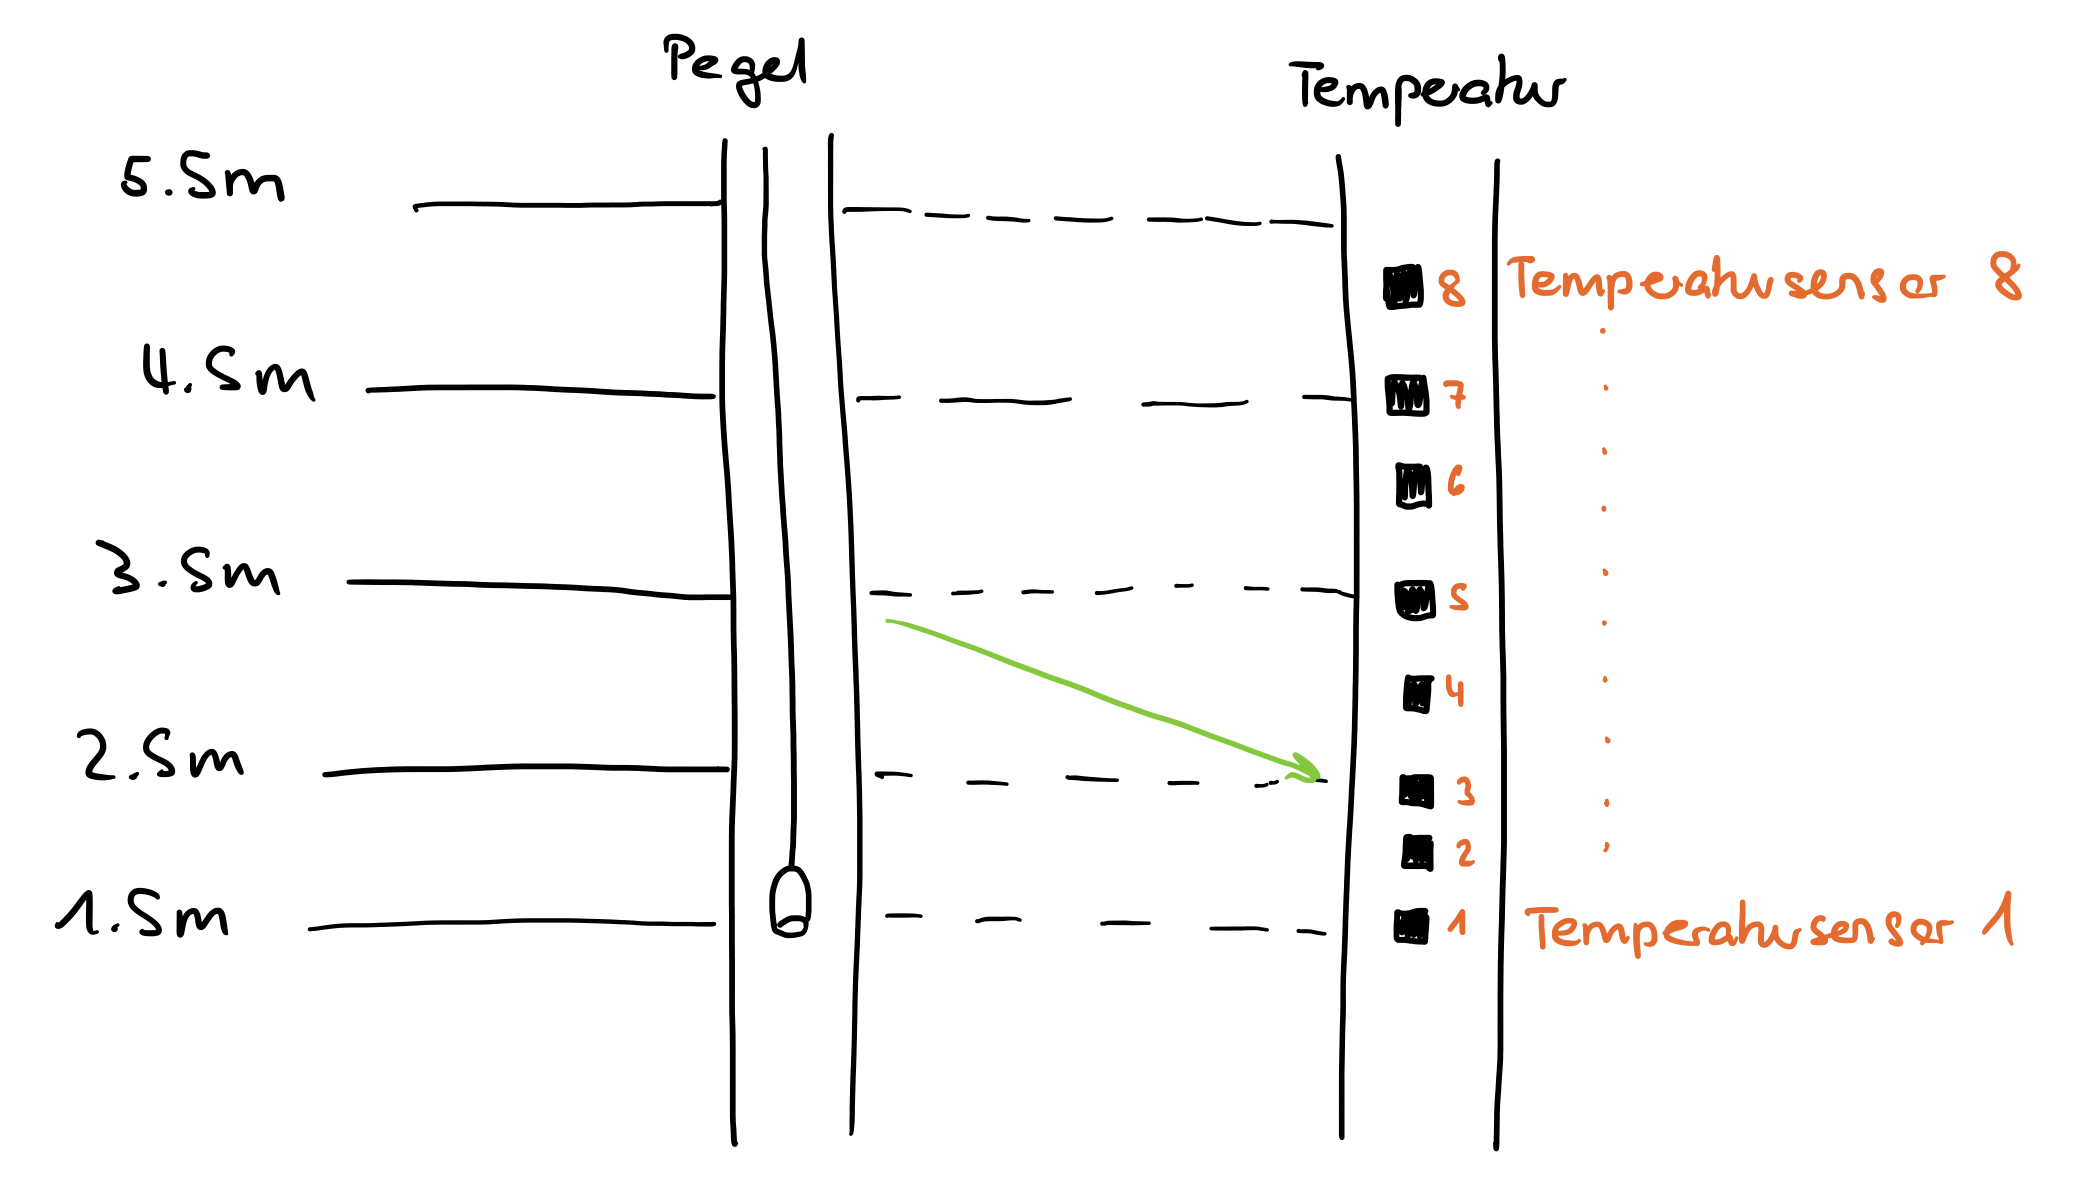
\includegraphics[width=0.9\linewidth]{img/wassertempsensoren.png}
	\caption{Zusammenhang zwischen Pegel und PT100-Temperaturwiderständen}
	\label{img:wassertempsensoren}
\end{figure}
